\documentclass[a4paper]{article}

\usepackage[utf8]{inputenc}
\usepackage[T1]{fontenc}
\usepackage[frenchb]{babel}
\usepackage{colortbl}
\usepackage{graphicx}
\usepackage{moresize}
\usepackage{anyfontsize}
\usepackage{hyperref}
\usepackage{longtable}
\usepackage[table]{xcolor}
\usepackage{tabularx}
\usepackage{pdfpages}
\usepackage{pdflscape}
\usepackage{lastpage}
\usepackage{array}
 \usepackage{float}
\usepackage{caption}
\usepackage{wrapfig}

% Definition des pages
\usepackage[left=3cm,right=3cm,top=3cm,bottom=3cm]{geometry}

% En-tete de page
\usepackage{fancyhdr}
\pagestyle{fancy}

% Lien hypertexte
\usepackage{hyperref}
\hypersetup{
  hidelinks,
  backref=true,
  pagebackref=true,
  hyperindex=true,
  colorlinks=false,
  breaklinks=true,
  urlcolor=ocre,
  bookmarks=true,
  bookmarksopen=false,
  pdftitle={Compte Rendu JEE},
  pdfauthor={Yohann HENRY - Jérémie PANTIN}
}

\definecolor{purp}{RGB}{110, 40, 150}
\definecolor{grisC}{RGB}{245, 245, 245}
\definecolor{grisF}{RGB}{224, 224, 224}
\definecolor{grisP}{RGB}{136, 136, 136}
\definecolor{ocre}{RGB}{51,102,0}

\makeatletter
\renewcommand{\@seccntformat}[1]{\llap{\textcolor{purp}{\csname the#1\endcsname}\hspace{1em}}}                    
\renewcommand{\section}{\@startsection{section}{1}{\z@}
{-4ex \@plus -1ex \@minus -.4ex}
{1ex \@plus.2ex }
{\normalfont\large\sffamily\bfseries}}
\renewcommand{\subsection}{\@startsection {subsection}{2}{\z@}
{-3ex \@plus -0.1ex \@minus -.4ex}
{0.5ex \@plus.2ex }
{\normalfont\sffamily\bfseries}}
\renewcommand{\subsubsection}{\@startsection {subsubsection}{3}{\z@}
{-2ex \@plus -0.1ex \@minus -.2ex}
{.2ex \@plus.2ex }
{\normalfont\small\sffamily\bfseries}}                        
\renewcommand\paragraph{\@startsection{paragraph}{4}{\z@}
{-2ex \@plus-.2ex \@minus .2ex}
{.1ex}
{\normalfont\small\sffamily\bfseries}}

\renewcommand\headrulewidth{1pt}
\fancyhead[L]{
\includegraphics[height=1cm]{resources/univ.png}}
\fancyhead[C]{Compte Rendu\\ \color{grisP}\texttt{Projet JEE}}
\fancyfoot[C]{\texttt{\thepage/\pageref{LastPage}}}
\makeatletter
\newcommand{\resetHeadWidth}{\fancy@setoffs}
\makeatother


\renewcommand{\arraystretch}{1.5}

\begin{document}

\begin{titlepage}
	\begin{center}
		{\fontsize{22}{30}\selectfont Projet Architectures Orientées Services sous JEE\\Guide d'utilisation}\\[\baselineskip]
		\vspace*{10pt}
		{\Large\itshape 19/01/2017}\\
		\vfill
		\rule{0.6\textwidth}{0.4pt}\\[\baselineskip]
		\begin{table}[h]
			\centering
			\def\arraystretch{1.4}
			\begin{tabular}{ll|ll}
				Yohann & HENRY & Jérémie & PANTIN\\
			\end{tabular}
		\end{table}
	\end{center}
\end{titlepage}

\thispagestyle{empty}

\tableofcontents
\newpage
\setcounter{page}{1}
\vspace*{0.5cm}

\section{Introduction}
Nous allons ici faire une brève présentation des demandes fournies dans l'intitulé du projet. Il faut noter que la technologie utilisée pour la partie Front est Thymeleaf.

\section{Identification sur le système}
\subsection{Inscription}
\begin{figure}[h]
\centering
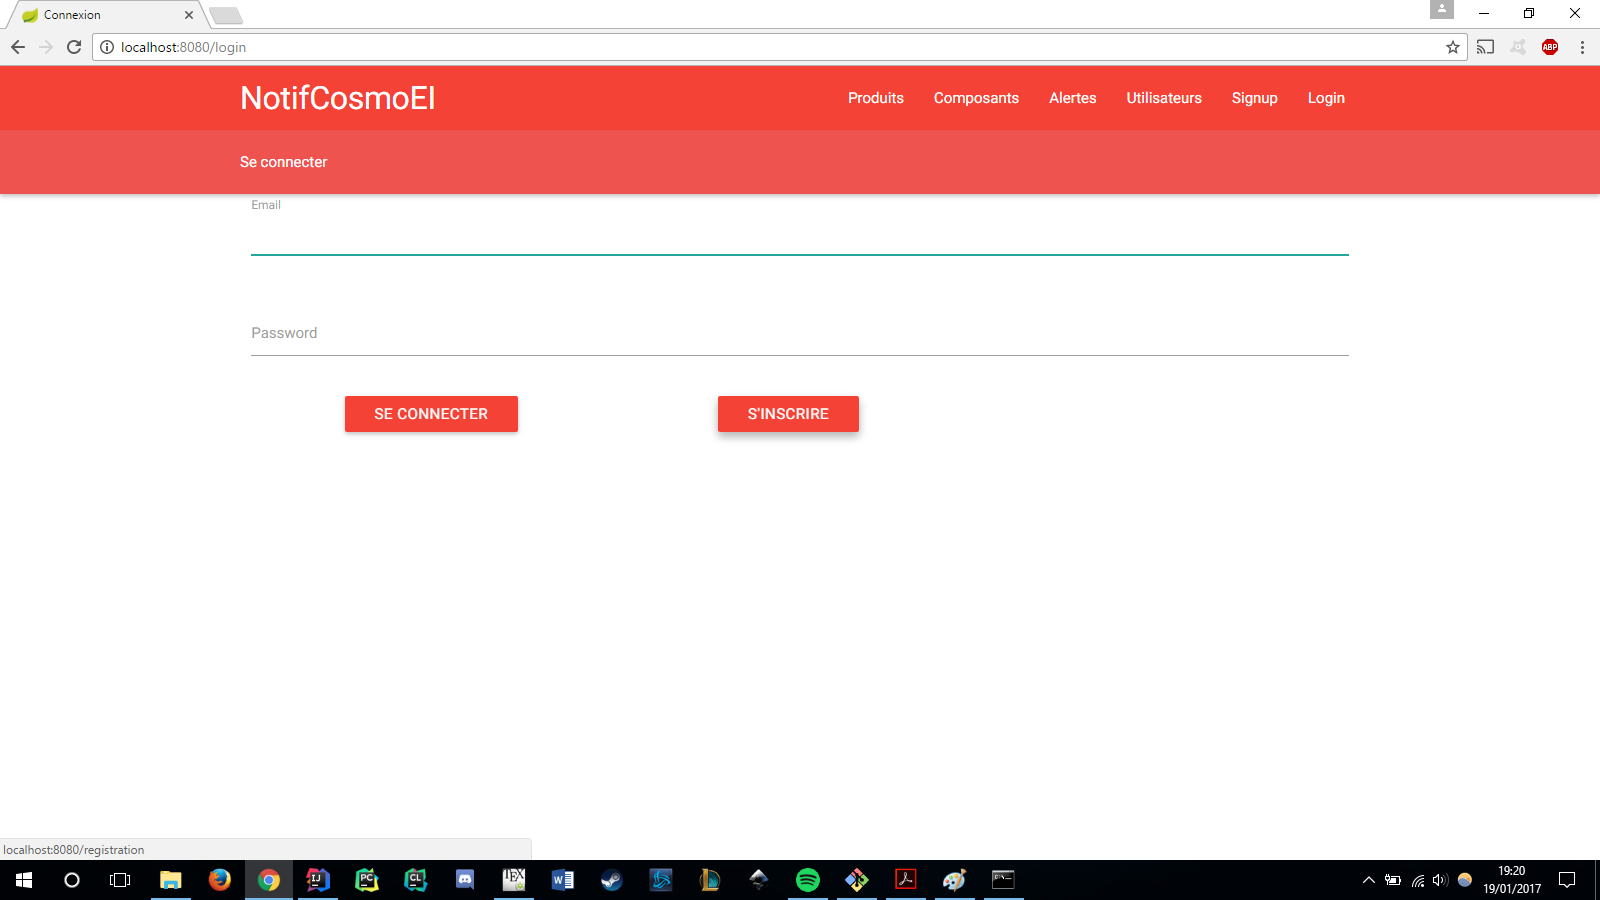
\includegraphics[scale=.35]{resources/inscription1.png}
\caption{Aller sur la page d'inscription}
\end{figure}

\begin{figure}[h]
\centering
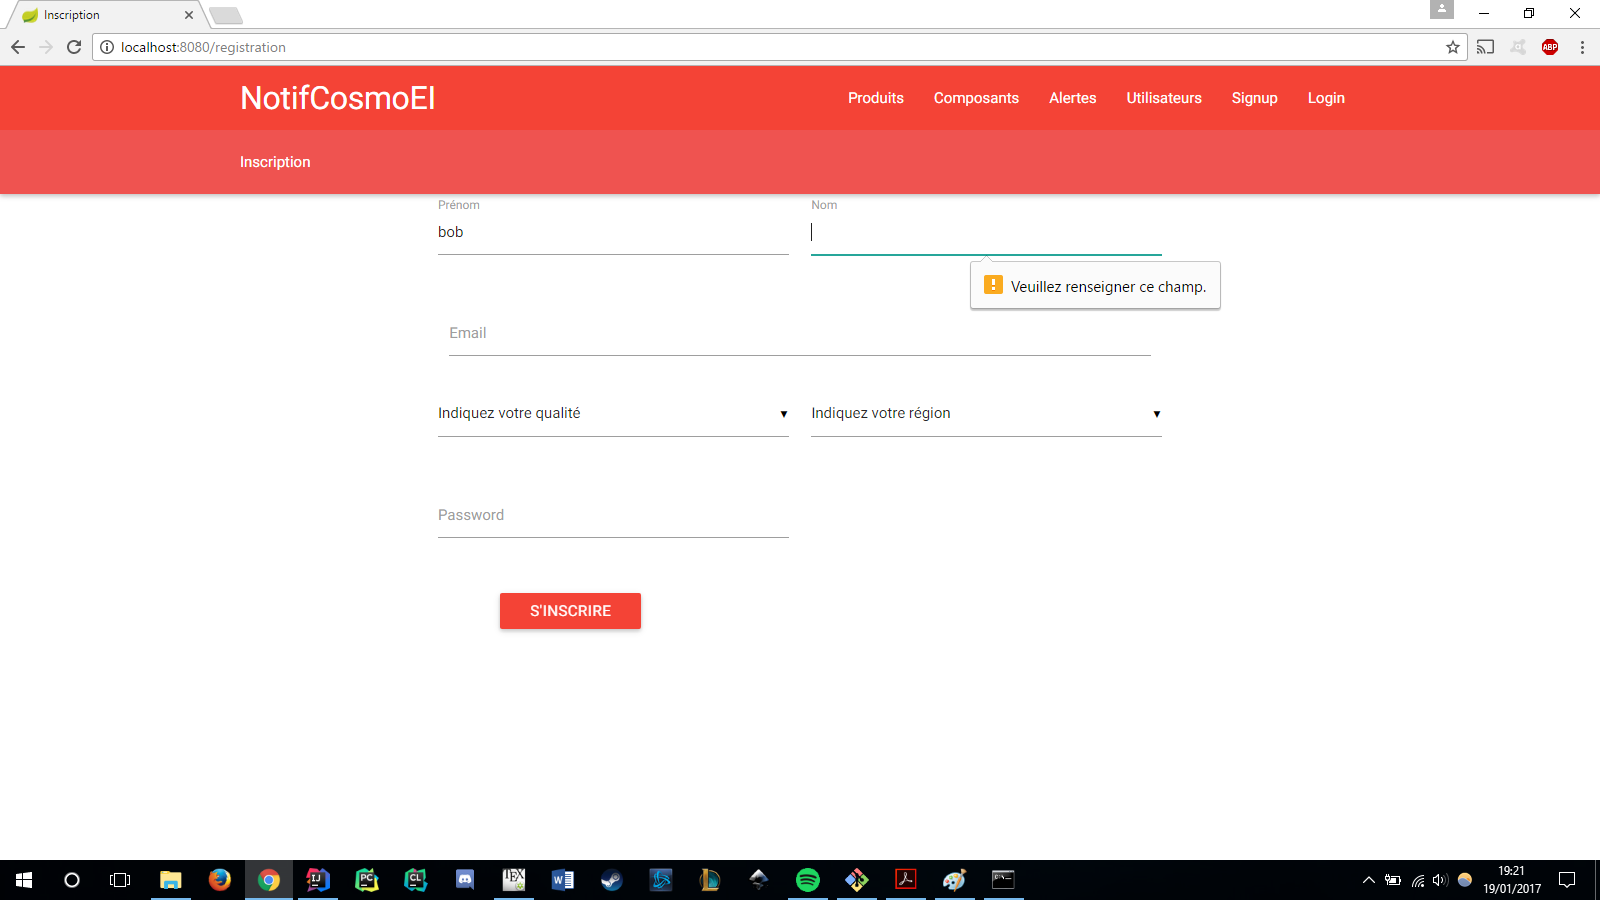
\includegraphics[scale=.35]{resources/inscription2.png}
\caption{Si non respect du formulaire}
\end{figure}

\begin{figure}[h]
\centering
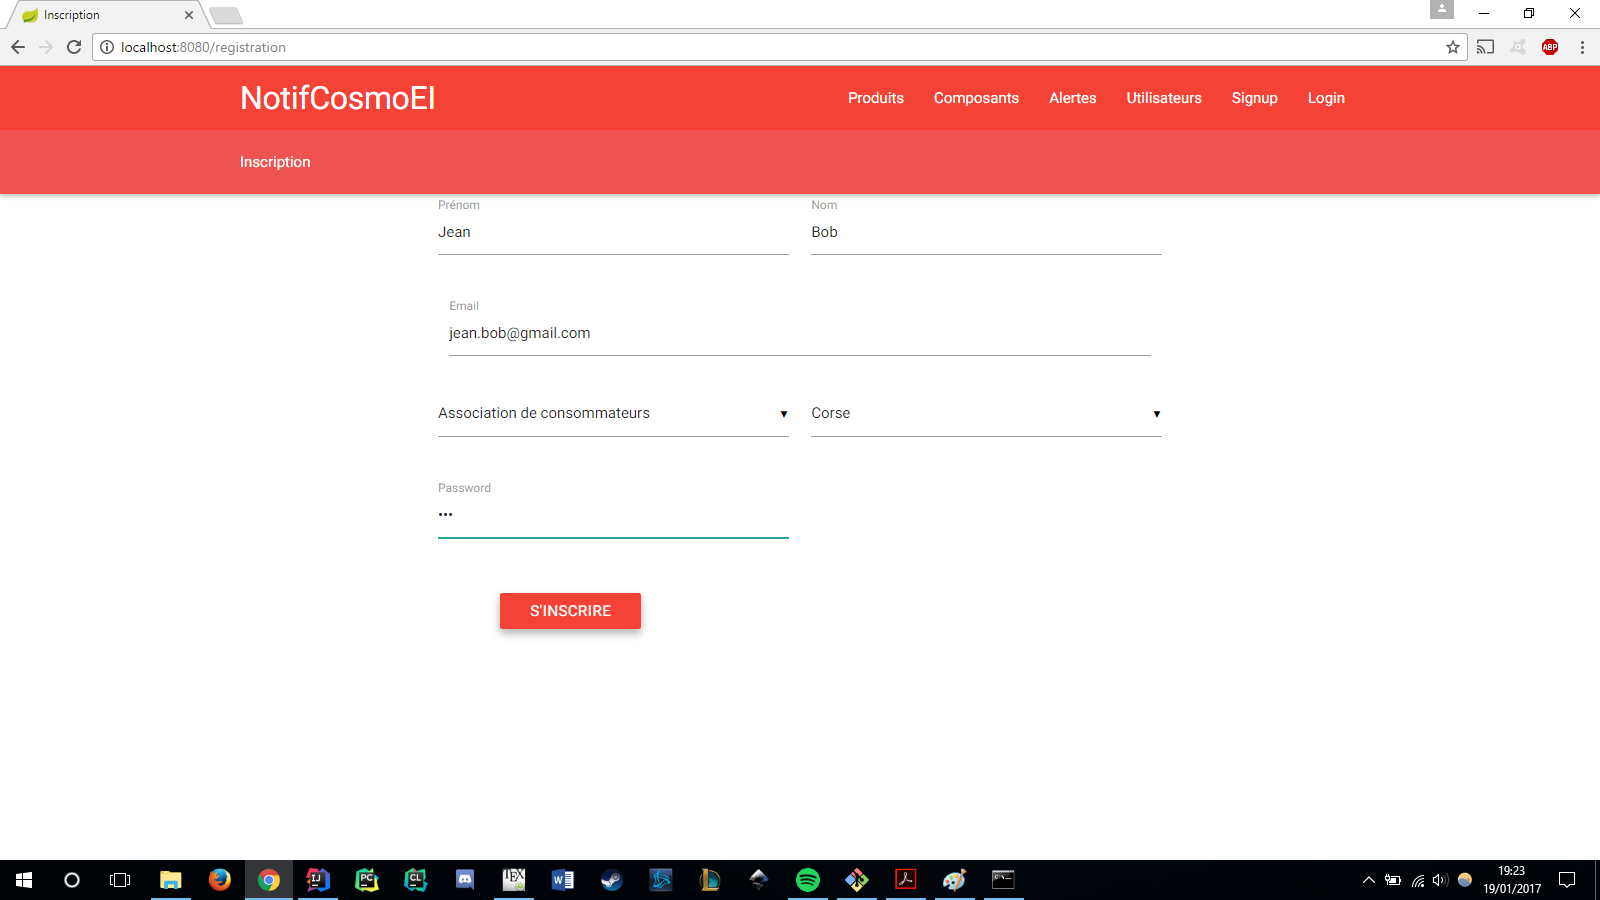
\includegraphics[scale=.35]{resources/inscription3.png}
\caption{Une inscription valide}
\end{figure}

\subsection{Connexion}
\begin{figure}[h]
\centering
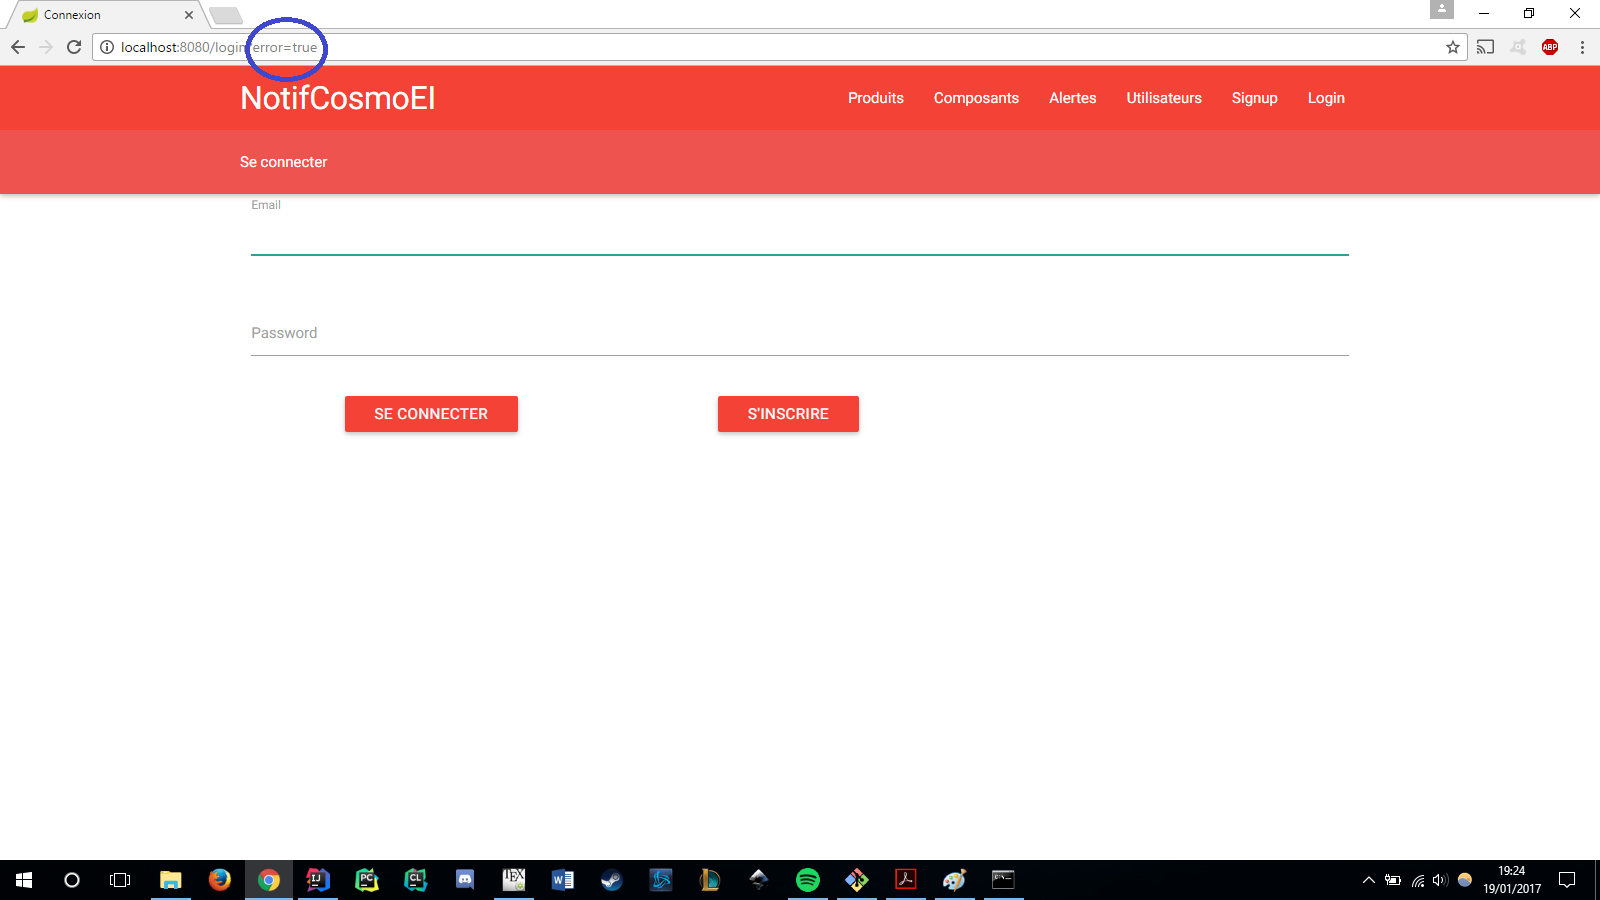
\includegraphics[scale=.35]{resources/connexion1.png}
\caption{Connexion avec un mauvais mot de passe}
\end{figure}

\begin{figure}[h]
\centering
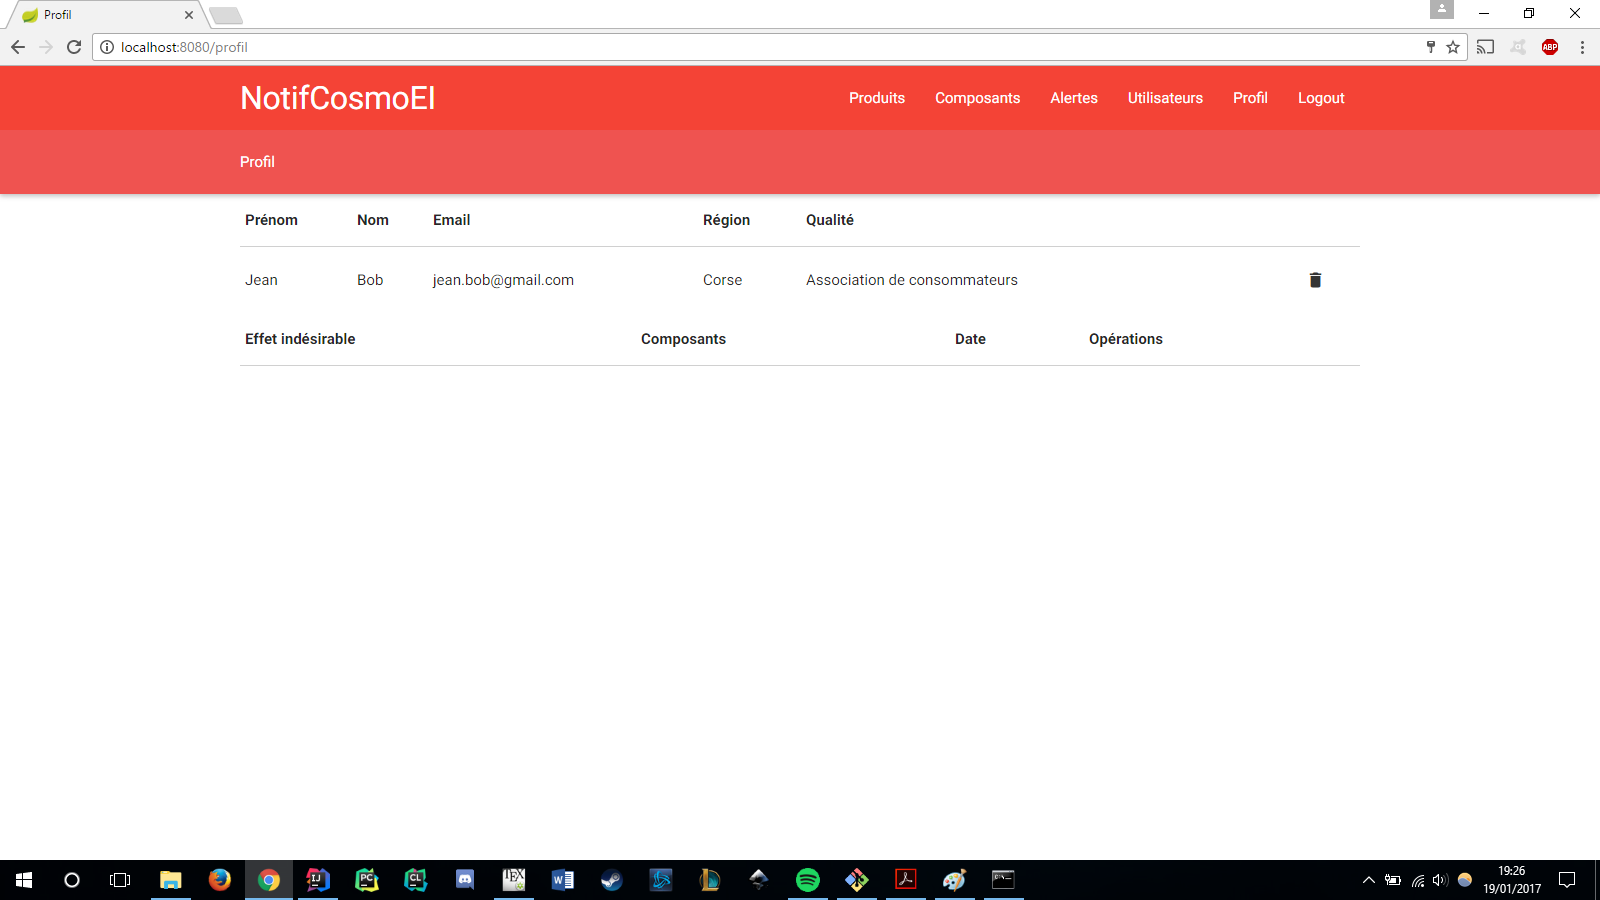
\includegraphics[scale=.35]{resources/connexion2.png}
\caption{Une fois la connexion, redirigé vers la page de profil}
\end{figure}

\section{CRUD}
\subsection{Read}
\begin{figure}[h]
\centering
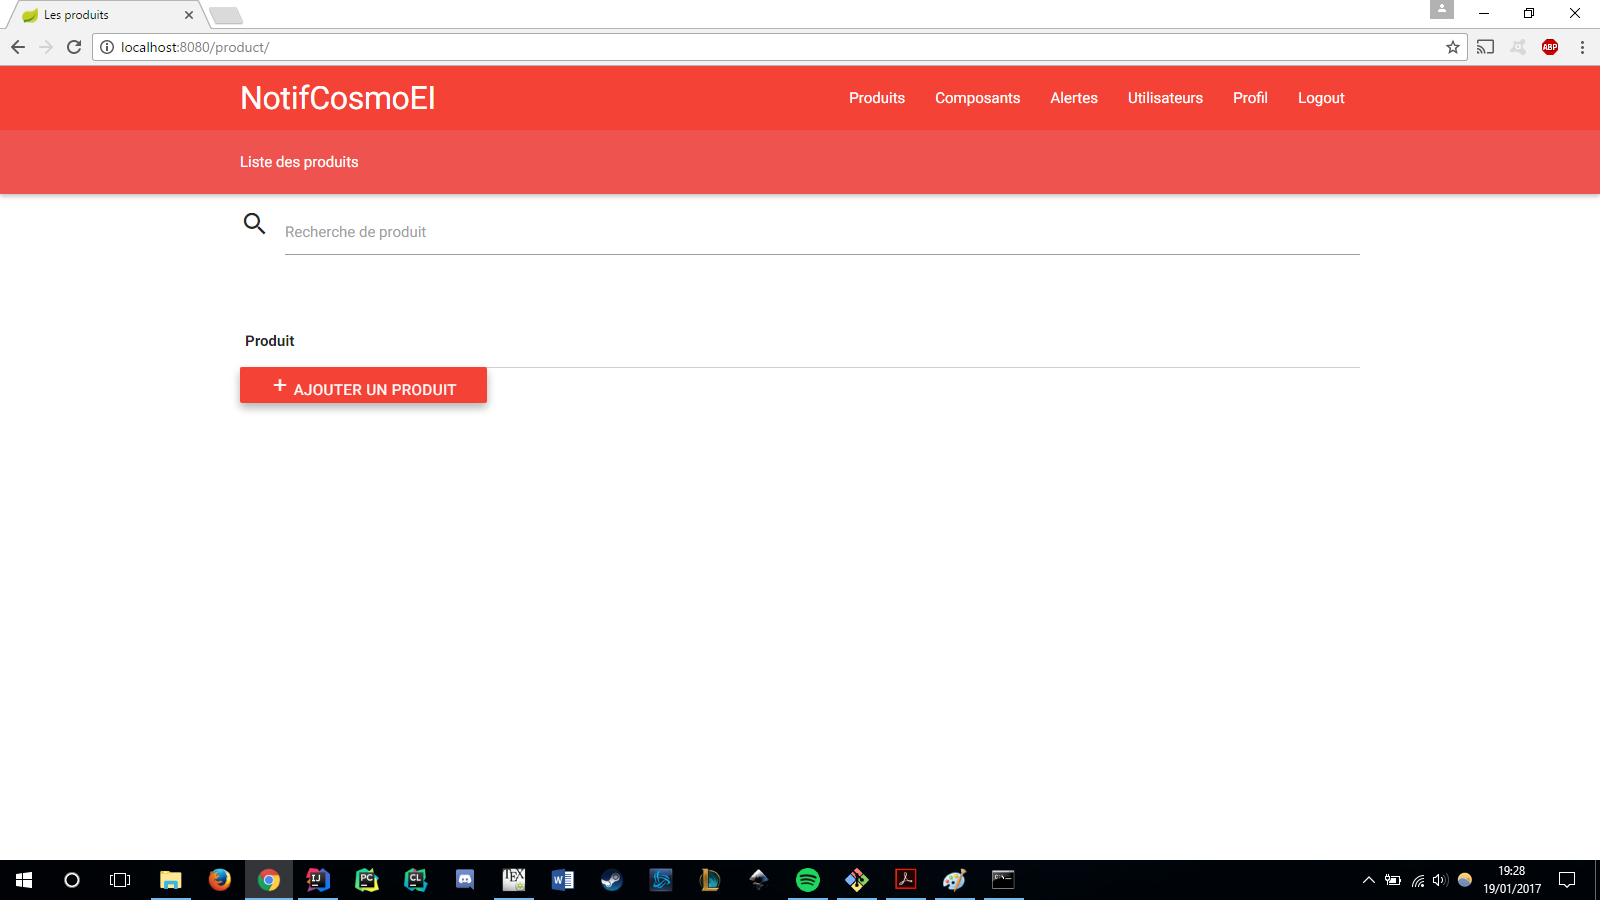
\includegraphics[scale=.35]{resources/get1.png}
\caption{GET sur un produit}
\end{figure}

\subsection{Create}
\begin{figure}[h]
\centering
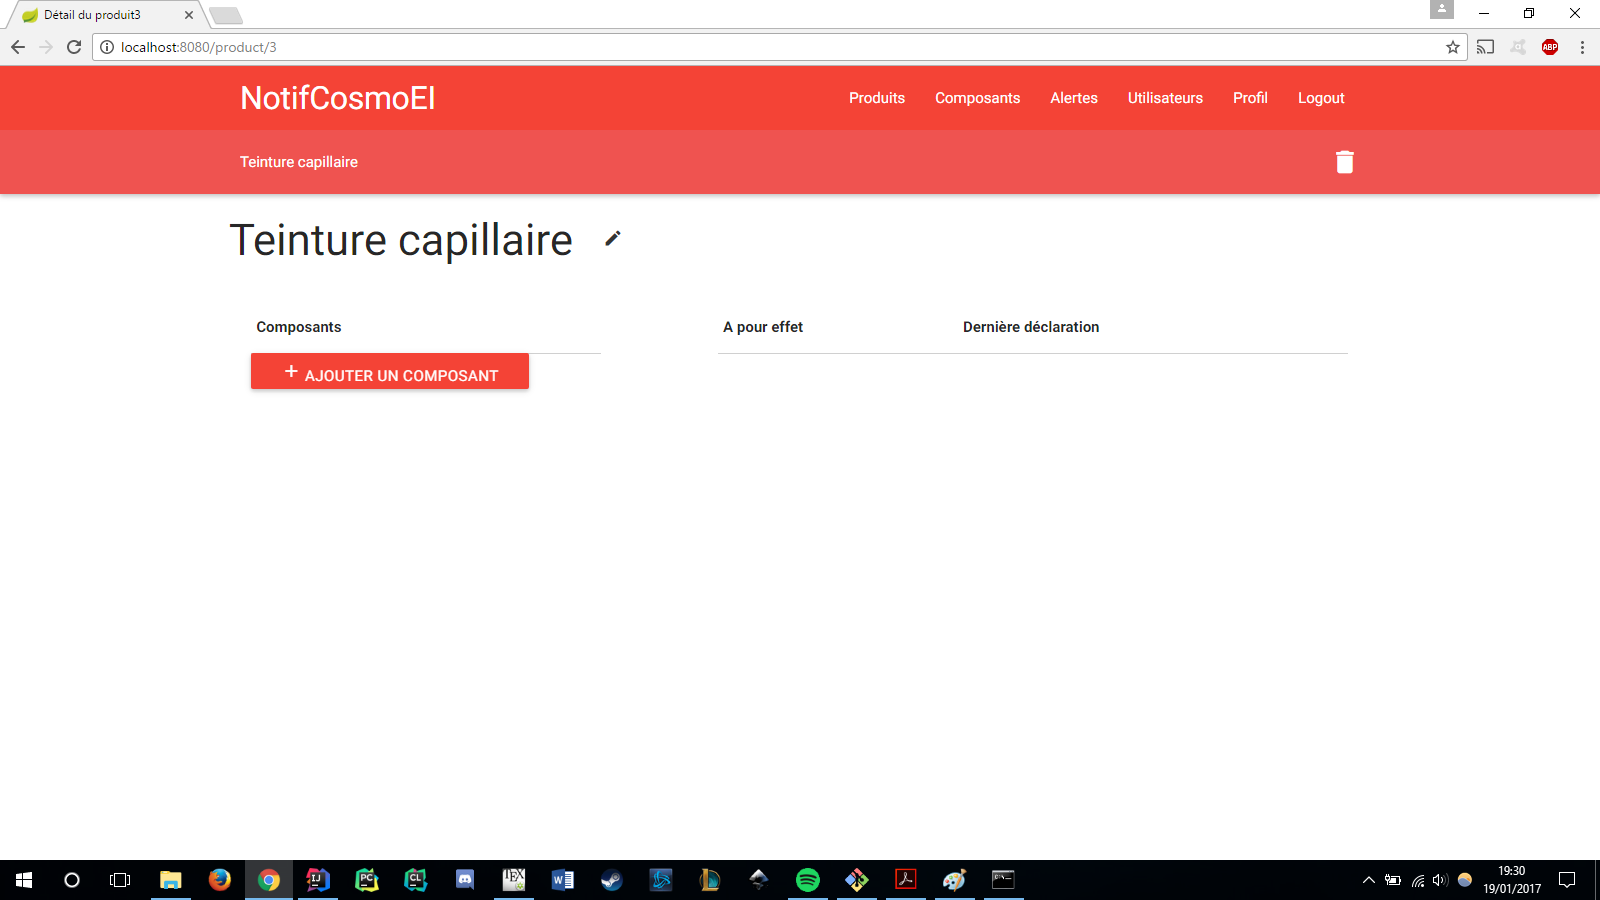
\includegraphics[scale=.35]{resources/get2.png}
\caption{Ajout d'un produit}
\end{figure}

\begin{figure}[h]
\centering
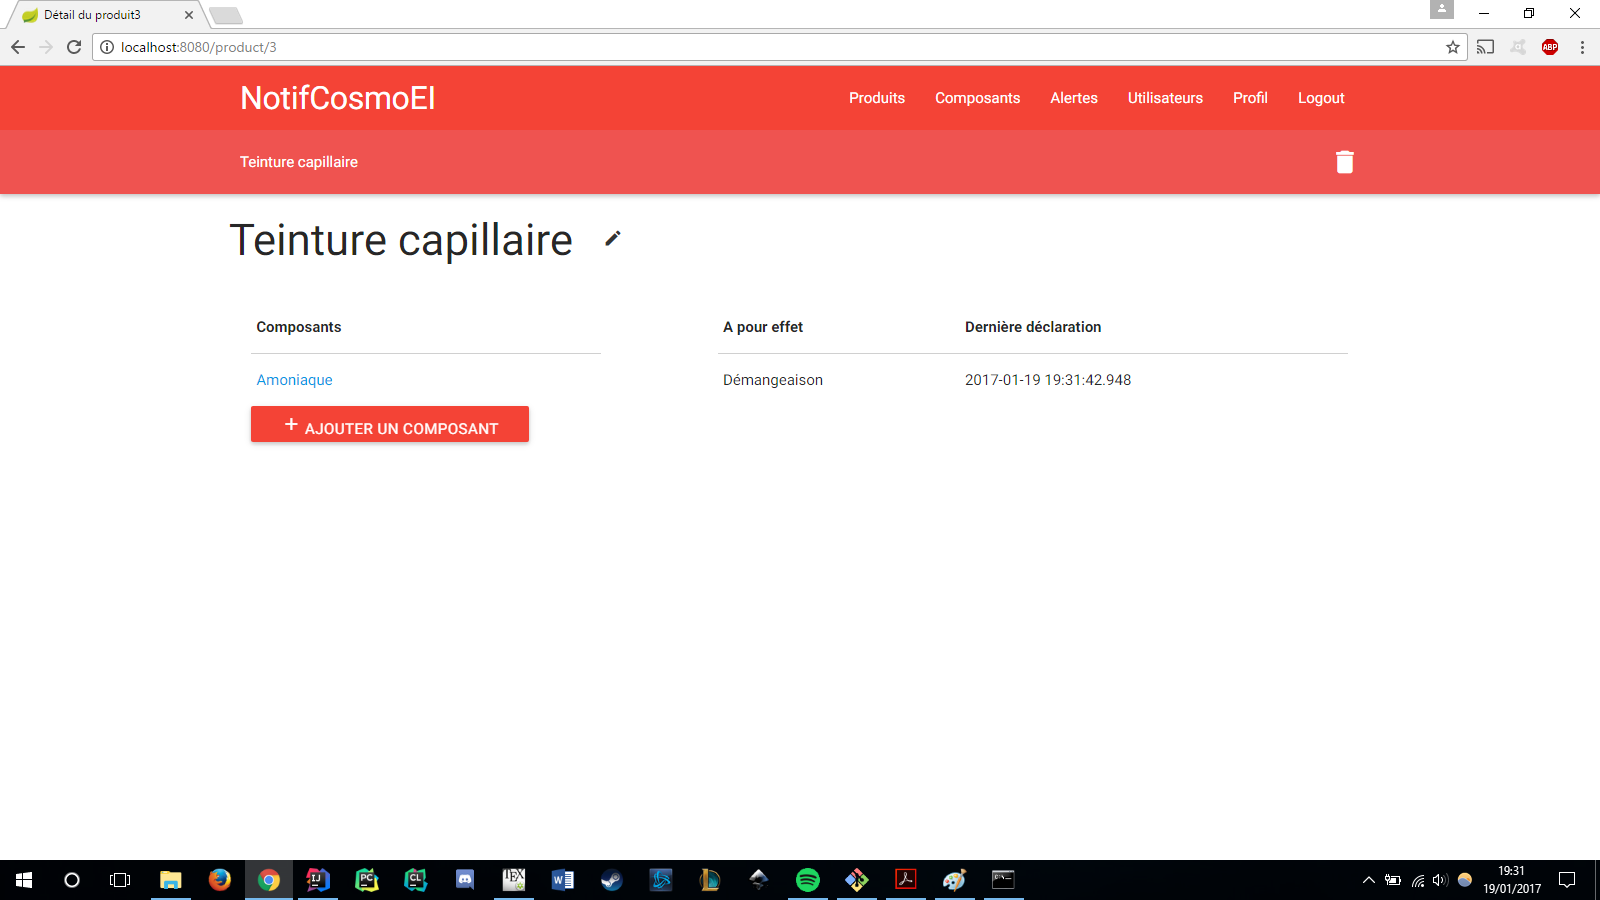
\includegraphics[scale=.35]{resources/get3.png}
\caption{Ajout d'un composant}
\end{figure}

\subsection{Delete}
\begin{figure}[h]
\centering
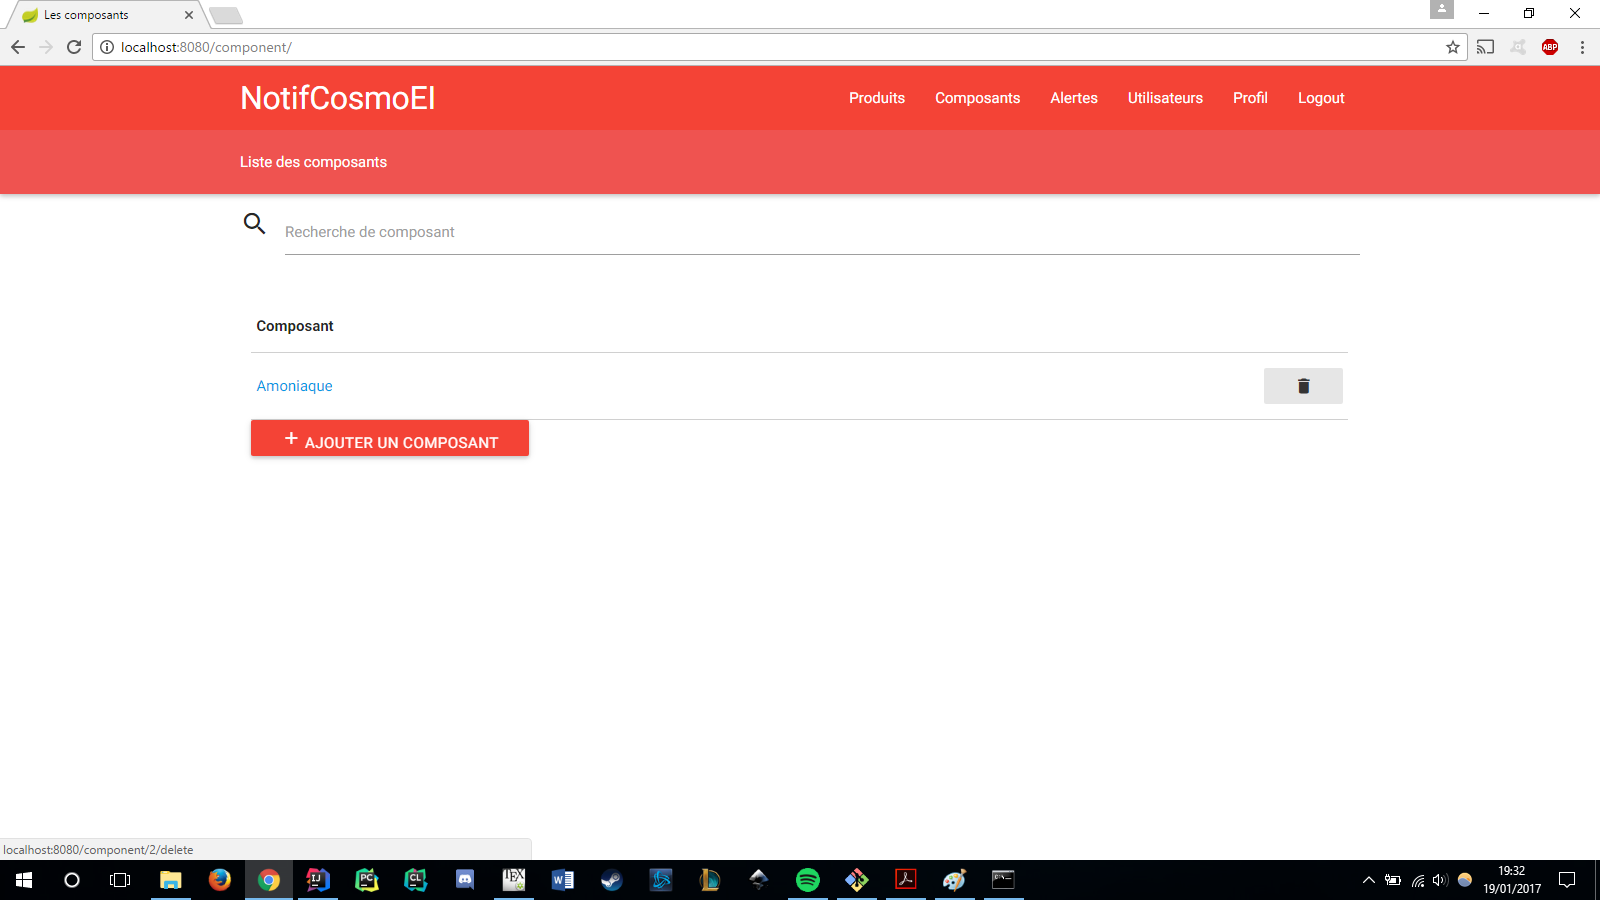
\includegraphics[scale=.35]{resources/get4.png}
\caption{Suppression d'un composant}
\end{figure}

\begin{figure}[h]
\centering
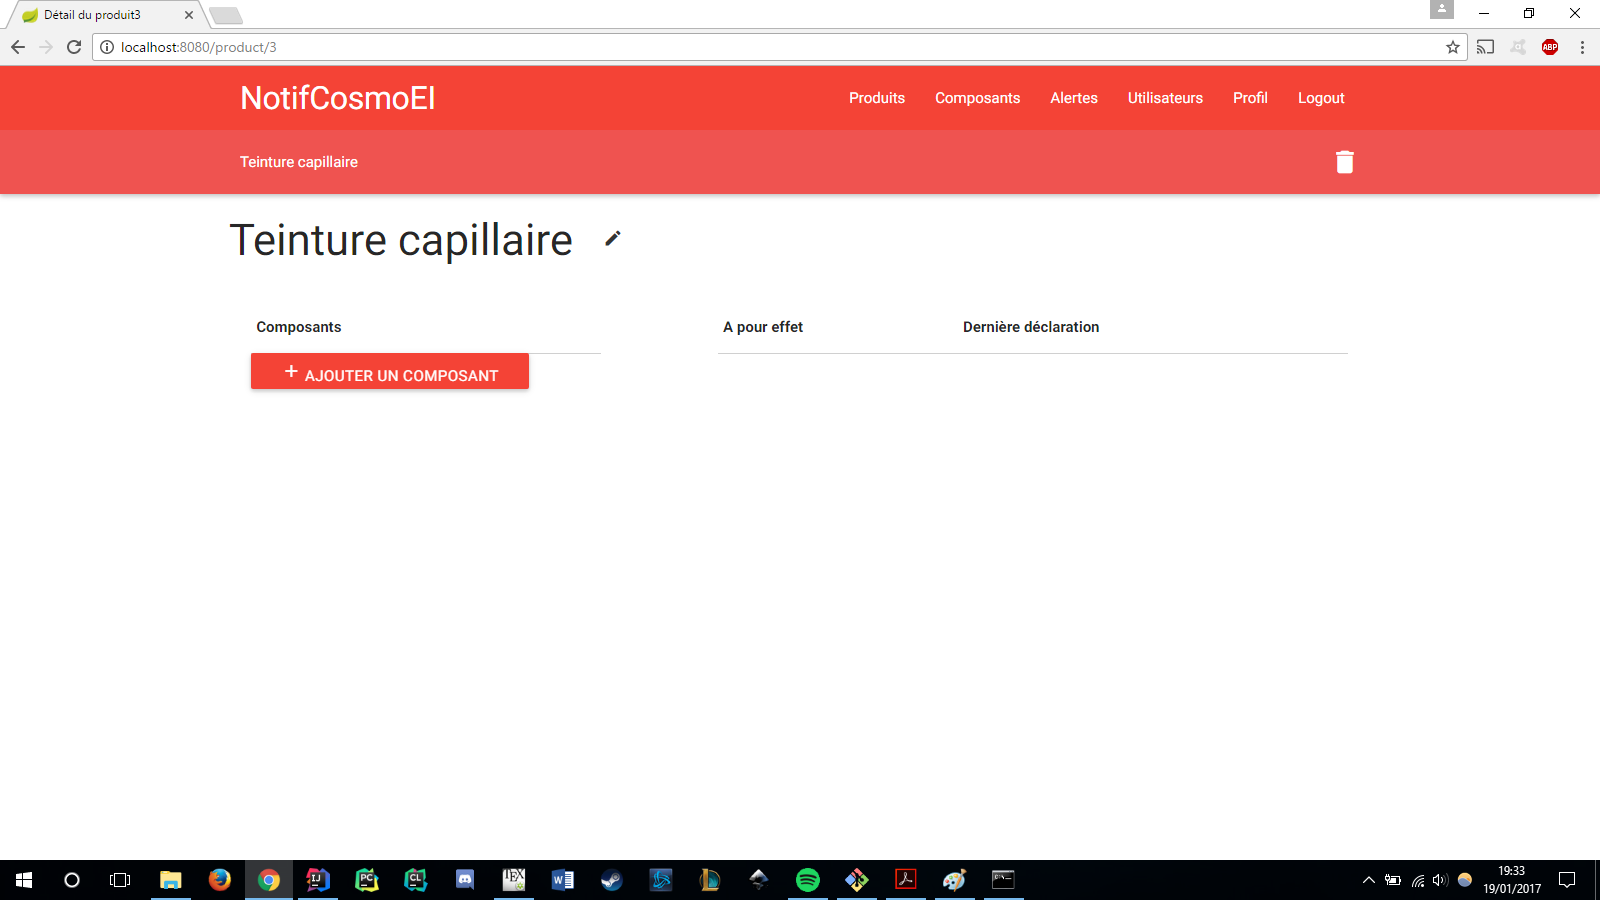
\includegraphics[scale=.35]{resources/get5.png}
\caption{Vérification de la suppression}
\end{figure}

\subsection{Update}
\begin{figure}[h]
\centering
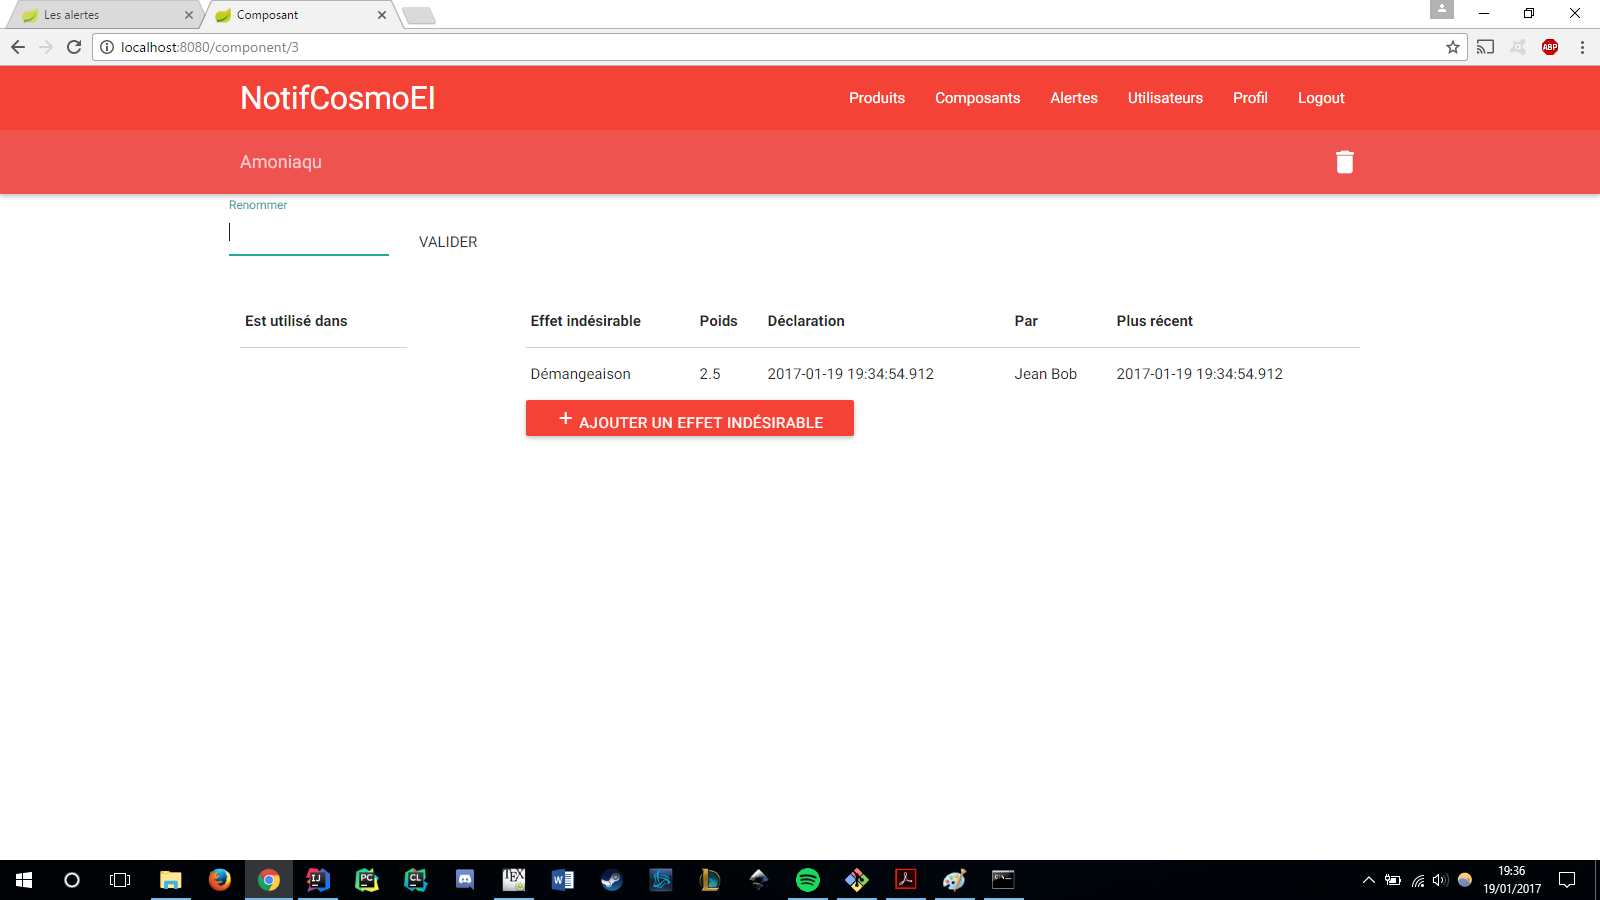
\includegraphics[scale=.35]{resources/get6.png}
\caption{Modification du nom d'amoniaque}
\end{figure}

\section{Alerte}
\begin{figure}[h]
\centering
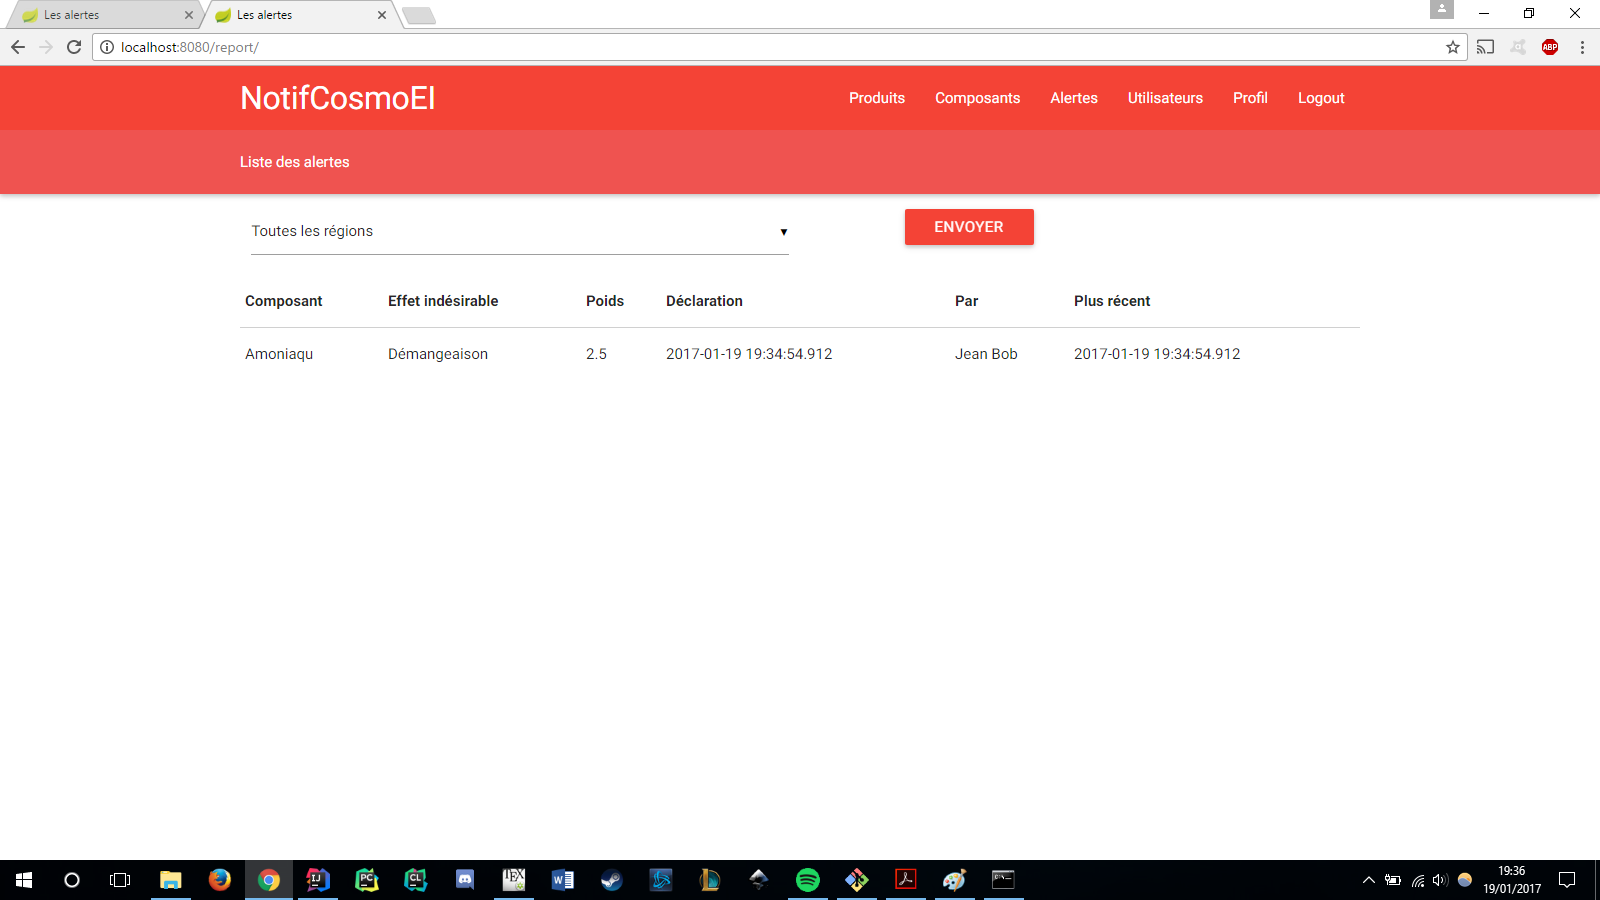
\includegraphics[scale=.35]{resources/alerte.png}
\caption{Alerte}
\end{figure}

\end{document}